\documentclass[11pt,a4paper]{article}
\usepackage[margin=2.5cm]{geometry}
\usepackage{amsmath,amssymb,amsthm}
\usepackage{booktabs}
\usepackage{xcolor}
\usepackage{tikz}
\usetikzlibrary{arrows.meta,positioning,fit,backgrounds,calc,shapes.geometric}
\usepackage[colorlinks=true,linkcolor=blue!50!black,urlcolor=blue!50!black,
            citecolor=blue!50!black]{hyperref}
\usepackage{enumitem}

\title{Branch and price for the 3D-SCPTOP\\[4pt]
\large theory, this implementation, and where to read further}
\author{}
\date{}

\newcommand{\conv}{\operatorname{conv}}
\newtheorem{observation}{Observation}

\begin{document}
\maketitle

\begin{abstract}
\noindent This note explains the branch-and-price method behind
MATH-3D-SCPTOP: the general theory it rests on, the specific choices made in
this implementation and why each was necessary, and a reading list for anyone
who wants the underlying material properly. It contains no computational
results --- those belong in the experimental sections of the paper --- and is
meant to be readable on its own.
\end{abstract}

\tableofcontents

\section{Why decompose at all}

The compact formulation of 3D-SCPTOP decides, simultaneously, what to procure,
what to hold, how many trucks to dispatch, and precisely how each truck is
loaded. The loading part is the difficulty. Placing containers on a truck floor
without overlap, stacking them within a height budget, respecting a per-stack
crush limit and a payload cap, is already an NP-hard packing problem, and the
compact model must carry one copy of it \emph{per truck it might dispatch}. The
model therefore grows with the fleet, and --- worse --- it grows in exactly the
part that is hardest to solve.

Two symptoms follow. The linear relaxation is weak, because a fractional truck
can be loaded fractionally and the packing constraints stop biting. And the
model is highly symmetric: trucks are interchangeable, so the same plan appears
in the search under an enormous number of relabellings, and branch and bound
re-derives it again and again.

Dantzig--Wolfe decomposition addresses both by changing the unit of decision.

\section{The Dantzig--Wolfe reformulation}

Instead of deciding where each container sits, we decide \emph{which complete
truck loads to dispatch}. Let $P^{g}$ be the set of all loads that a truck
travelling in direction $g$ could legally carry: every element of $P^{g}$ is a
fully specified, geometrically realisable load. Write $a^{p}_{c}$ for the number
of units of commodity $c$ that load $p$ carries.

The master problem chooses non-negative integers $\lambda^{g}_{pt}$ --- how many
trucks of load $p$ leave in period $t$ --- subject to the inventory and demand
constraints, minimising transport plus inventory cost. Three things change at
once:

\begin{itemize}[leftmargin=1.4em]
\item \textbf{The packing constraints disappear from the master.} They are not
relaxed; they are enforced inside the definition of $P^{g}$. Any $p$ the master
can use is loadable by construction.
\item \textbf{The relaxation is stronger.} The master's linear relaxation
optimises over $\conv(P^{g})$ rather than over the linear description of the
packing polytope, and the former is contained in the latter. Convexification is
where the bound improvement comes from.
\item \textbf{The symmetry collapses.} Identical trucks become one variable with
a count, not many variables to permute.
\end{itemize}

The price is that $P^{g}$ is astronomically large. We never write it down.

\section{Column generation}

We solve a \emph{restricted} master (RMP) over a subset
$\bar P^{g}\subseteq P^{g}$, read its dual prices, and ask a subproblem whether
any load outside $\bar P^{g}$ would improve it. The reduced cost of a load $p$
in period $t$ has the shape
\[
  \bar c(p,t) \;=\; cK \;-\; \sum_{c}\pi_{ct}\,a^{p}_{c} \;-\; \nu_{gt},
\]
with $\pi$ the duals of the linking constraints and $\nu$ the dual of the fleet
row. Finding the most negative reduced cost means solving
\[
  \zeta_{gt}\;=\;\max_{p\in P^{g}}\ \sum_{c}\pi_{ct}\,a^{p}_{c},
\]
which is the \emph{pricing subproblem}: design one truck load of maximum
dual-weighted value, subject to all the geometry. If $\zeta_{gt}\le cK-\nu_{gt}$
for every direction and period, no load prices out and the RMP has solved the
full master linear programme. Otherwise the improving load is added and the
cycle repeats.

\begin{figure}[h!]
\centering
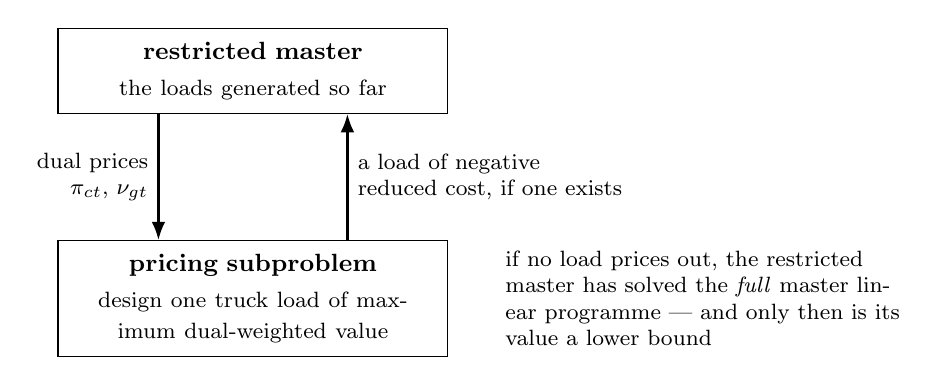
\begin{tikzpicture}[>=Latex, font=\small, node distance=8mm,
  b/.style={rectangle, draw, fill=white, text width=46mm, align=center,
            inner sep=5pt}]
  \node[b] (rmp) {\textbf{restricted master}\\[2pt]
     \footnotesize the loads generated so far};
  \node[b, below=16mm of rmp] (pp) {\textbf{pricing subproblem}\\[2pt]
     \footnotesize design one truck load of maximum dual-weighted value};
  \draw[->, thick] ([xshift=-12mm]rmp.south) -- ([xshift=-12mm]pp.north)
        node[midway, left, align=right, font=\footnotesize]
        {dual prices\\ $\pi_{ct}$, $\nu_{gt}$};
  \draw[->, thick] ([xshift=12mm]pp.north) -- ([xshift=12mm]rmp.south)
        node[midway, right, align=left, font=\footnotesize]
        {a load of negative\\ reduced cost, if one exists};
  \node[align=left, font=\footnotesize, right=6mm of pp.east, text width=52mm]
       {if no load prices out, the restricted master has solved the
        \emph{full} master linear programme --- and only then is its value a
        lower bound};
\end{tikzpicture}
\caption{Column generation. The subproblem is a separation problem in the dual:
it looks for a violated dual constraint.}
\end{figure}

Two practical facts about this loop matter later. It \emph{tails off}: the last
iterations buy progressively less objective value while costing a full
subproblem solve each. And the master is typically \emph{degenerate}, so the
duals jump between vertices from one iteration to the next rather than settling
smoothly --- which is why an iteration returning nothing is not evidence that
the loop has converged.

\section{What the master's value is, and is not}

This is the single most misused quantity in the method, so it is worth stating
carefully.

\begin{observation}
The restricted master optimises over a \emph{subset} of the columns, so its
optimal value is an \textbf{upper} bound on the master linear programme's value,
not a lower bound on anything. It becomes a lower bound on the integer optimum
only once column generation has converged --- and \emph{converged} means proved,
not merely observed.
\end{observation}

Two bounds are therefore available, and they differ in what they require.

\paragraph{The certified bound.} If the subproblem \emph{proves}
$\zeta_{gt}\le cK-\nu_{gt}$ for every $g$ and $t$, then the current duals are
feasible for the dual of the full master, weak duality applies, and the RMP
value is a valid lower bound on the integer optimum. This is the strong
statement, and it requires the packing subproblem to be closed to proven
optimality in every direction and period --- not merely to return nothing within
a time limit.

\paragraph{The Lagrangian bound.} When proof is unavailable, dualising the
linking constraints gives a bound of the form
\[
  z_{\mathrm{MP}} \;\ge\; z_{\mathrm{RMP}} \;+\; \bar X\cdot
  \min_{g,t}\min\{0,\;cK-\zeta_{gt}-\nu_{gt}\},
\]
valid at every iteration, converged or not. It is the Farley bound, and it has
two delicate ingredients. The value substituted for $\zeta_{gt}$ must be an
\emph{upper} bound on the subproblem's optimum --- the solver's dual bound, never
its incumbent --- so that a subproblem stopped early still yields a valid
verdict. And $\bar X$ must be a genuine bound on the number of trucks an optimal
solution dispatches; a crude choice makes the correction so pessimistic that the
bound is useless.

\paragraph{Where certificates go wrong.} Both bounds are only as good as the
exhaustiveness of the check behind them, and the failure modes are quiet ones.

\begin{itemize}[leftmargin=1.4em]
\item \emph{A pair never examined.} If the implementation skips a direction and
period on a shortcut argument --- for instance, that non-positive commodity
duals mean nothing there can pay for a truck --- the argument must be complete.
Non-positive duals bound $\sum_{c}\pi_{ct}a_{c}$ by zero, which settles the
reduced cost only when $cK-\nu_{gt}\ge 0$ as well. A pair skipped without that
second test contributes neither a proof nor an objection, and the certificate is
then claimed over something nobody looked at.
\item \emph{An empty answer read as a proof.} A subproblem that returns no
column because it ran out of time has proved nothing. Because the master is
degenerate, empty answers occur well before convergence, so this failure is
common rather than exotic.
\item \emph{A bound that understates the subproblem's optimum.} If pricing is
run with a threshold constraint and reports infeasibility, that proves no column
beats the threshold --- so the \emph{threshold} bounds $\zeta_{gt}$. Recording a
smaller value inflates the Lagrangian correction in the wrong direction.
\item \emph{Rounding the duals the wrong way.} Prices are irrational in general
and must be rounded before entering an integer-coefficient subproblem. Rounding
\emph{up} keeps the rounded objective dominating the true one, so the returned
bound over-estimates $\zeta_{gt}$, which is what both bounds require. Rounding
to nearest quietly invalidates the certificate.
\end{itemize}

All four push the reported bound in the same direction: upwards. A lower bound
that is too high is not a loose bound, it is a false statement, and every
optimality gap computed from it is wrong.

\section{Branching}

Column generation solves the master's relaxation. Reaching an integer solution
needs branching, and this is where branch and price departs most sharply from
ordinary branch and bound.

\paragraph{Why branching on the master's variables is a poor rule.} The obvious
choice is to fix a fractional $\lambda^{g}_{pt}$. It fails for two related
reasons. First, the master typically contains many columns that differ only in
detail, so forbidding one lets the relaxation shift the same fractional weight
onto a near-identical neighbour; the search descends without the relaxation ever
becoming integral. Second, the decision is hard to enforce in the subproblem:
excluding one specific load from $P^{g}$ turns a clean packing problem into a
packing problem with an awkward side constraint, and repeated exclusions
accumulate into something the oracle can no longer solve efficiently.

\paragraph{Branching on original variables.} The standard remedy is to branch on
quantities of the \emph{original} formulation, recovered from the master
solution. Such a quantity has no symmetric twin, and a bound on it is a bound on
a row that already carries a dual, so the subproblem keeps its structure and
merely sees a different price. Ryan and Foster's rule for set-partitioning
masters --- branch on whether two items travel together --- is the classical
instance of this idea; Vanderbeck's generic schemes extend it to masters whose
subproblem solutions are not binary.

\paragraph{The hierarchy used here.} This implementation branches on the
shallowest level that is fractional:
\begin{enumerate}[leftmargin=1.6em]
\item the number of dispatches in a direction and period, which is integral in
every feasible plan and whose row contains every column of that period;
\item the delivered quantities per commodity and period, which count physical
units and are integral in any plan although the relaxation leaves them
continuous;
\item a column variable, only when the first two are already integral.
\end{enumerate}
Both children of a branch are kept, and the open node with the cheapest
relaxation is expanded next, so a wrong first move is recovered instead of being
carried to the bottom of a dive.

\begin{figure}[h!]
\centering
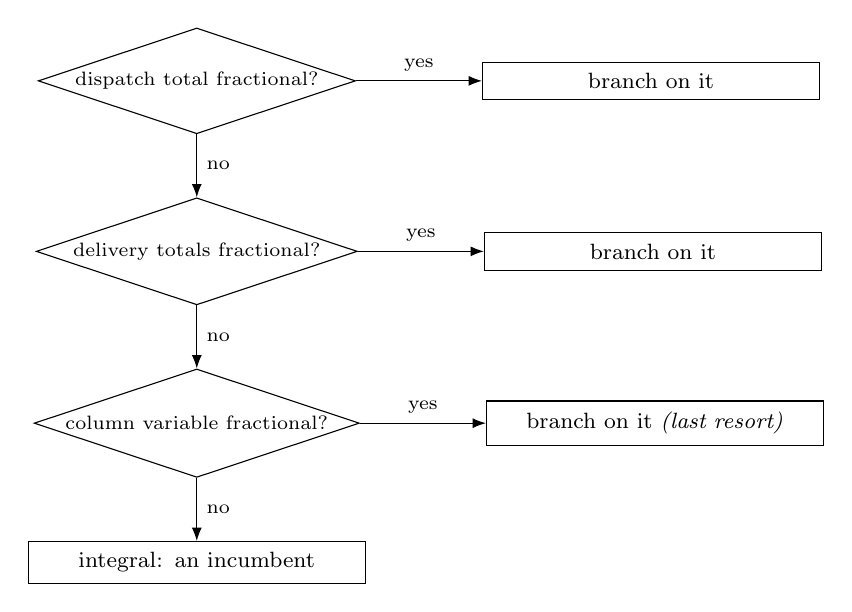
\begin{tikzpicture}[>=Latex, font=\footnotesize, node distance=6mm,
  d/.style={diamond, aspect=3, draw, fill=white, inner sep=1pt, align=center,
            font=\scriptsize},
  r/.style={rectangle, draw, fill=white, align=center, inner sep=4pt,
            text width=40mm}]
  \node[d] (a) {dispatch total fractional?};
  \node[d, below=8mm of a] (b) {delivery totals fractional?};
  \node[d, below=8mm of b] (c) {column variable fractional?};
  \node[r, right=16mm of a] (a1) {branch on it};
  \node[r, right=16mm of b] (b1) {branch on it};
  \node[r, right=16mm of c] (c1) {branch on it \emph{(last resort)}};
  \node[r, below=8mm of c] (d1) {integral: an incumbent};
  \draw[->] (a) -- node[above,font=\scriptsize] {yes} (a1);
  \draw[->] (b) -- node[above,font=\scriptsize] {yes} (b1);
  \draw[->] (c) -- node[above,font=\scriptsize] {yes} (c1);
  \draw[->] (a) -- node[right,font=\scriptsize] {no} (b);
  \draw[->] (b) -- node[right,font=\scriptsize] {no} (c);
  \draw[->] (c) -- node[right,font=\scriptsize] {no} (d1);
\end{tikzpicture}
\caption{Branching on aggregates first. Each level is integral in any feasible
plan, so each dichotomy is valid; the levels differ in how much of the search
space each one actually partitions.}
\end{figure}

\paragraph{Pricing at the nodes.} Columns continue to be generated at every
node, under that node's branching bounds. This is what distinguishes branch and
price from \emph{price and branch}, where the pool is frozen once the root is
solved. It matters here for a reason particular to this problem, explained next.

\section{The geometry of the column set}

The pricing objective is linear in the load vector. Its optimum over $P^{g}$ is
therefore attained at an extreme point of $\conv(P^{g})$ --- for \emph{every}
dual vector, without exception.

\begin{observation}
A load that lies in the interior of $\conv(P^{g})$, dominated componentwise by a
convex combination of other loads, can never be returned by pricing, no matter
what the duals are.
\end{observation}

This is not a pathology; it is a property of linear objectives. But it has a
sharp consequence for a problem in which trucks are dispatched in whole numbers.
The relaxation is content with a dominated load: it buys a fractional
combination of the dominating extreme loads and pays for one truck. An integer
plan cannot do that --- it must pay for each of the trucks in the combination.
So the load an integer plan wants may be precisely the one column generation
will never produce.

Branching down is what breaks the deadlock. Forbidding a dominating column
removes it from the relaxation, which moves the duals, and the oracle is then
asked for a load that did not previously price out. The search is therefore not
merely a way of reaching integrality: it is a mechanism for generating columns
that no dual vector could have requested.

\begin{figure}[h!]
\centering
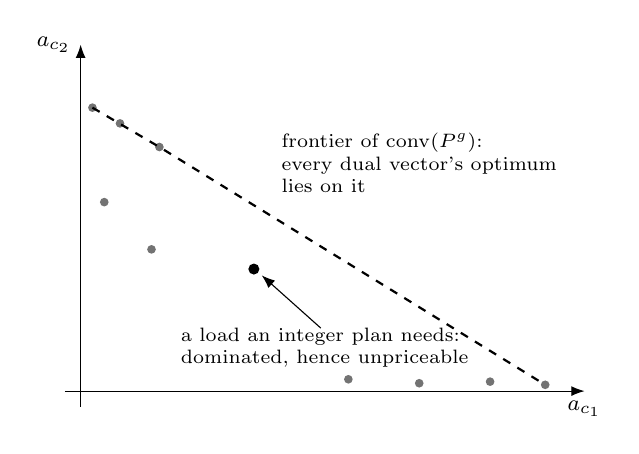
\begin{tikzpicture}[>=Latex, font=\footnotesize, scale=1.0]
  \draw[->] (-0.2,0) -- (6.4,0) node[below] {$a_{c_1}$};
  \draw[->] (0,-0.2) -- (0,4.4) node[left] {$a_{c_2}$};
  \foreach \p in {(0.15,3.6),(0.5,3.4),(1.0,3.1),(0.3,2.4),(0.9,1.8),
                  (3.4,0.15),(4.3,0.1),(5.2,0.12),(5.9,0.08)}
      \fill[black!55] \p circle[radius=0.055];
  \draw[dashed, thick] (0.15,3.6) -- (1.0,3.1) -- (5.9,0.08);
  \node[align=left, font=\scriptsize] at (4.3,2.9)
      {frontier of $\conv(P^{g})$:\\ every dual vector's optimum\\ lies on it};
  \fill[black] (2.2,1.55) circle[radius=0.07];
  \node[font=\scriptsize, anchor=west, align=left] at (1.15,0.55)
      {a load an integer plan needs:\\ dominated, hence unpriceable};
  \draw[->] (3.05,0.8) -- (2.3,1.47);
\end{tikzpicture}
\caption{Schematic, in two commodities. Dots are loads a sweep of price vectors
produces; all lie on the frontier, because that is where a linear objective is
maximised. A dominated load below the frontier is unreachable by pricing and may
nonetheless be the load a cheap integer plan requires.}
\end{figure}

The same observation applies to \emph{initialisation}. A pool built by solving
the subproblem under a family of demand-derived price vectors --- the aggregate
mix, per-period mixes, single-commodity vectors, random draws --- is extreme by
construction, however many vectors are tried. To obtain interior loads at all,
the oracle must be asked a different question: not ``which load maximises this
price vector'' but ``which loadable truck comes closest to this composition''.
That is a different objective over the same feasible set, and it is how this
implementation seeds interior loads.

\section{Primal solutions}

Branch and price is often poor at producing feasible solutions early: the
relaxation is fractional, and the tree may descend a long way before an integral
node appears. The standard remedy is a primal heuristic run periodically on the
current pool.

This implementation solves the master as an \emph{integer} programme over the
columns generated so far, at intervals during the search. It is cheap, because
the pool is small compared with the original formulation, and its solution
serves two purposes: it is a feasible plan in its own right, and it is the
incumbent against which nodes can be pruned. Without an incumbent, a best-first
search has nothing to prune with and its open list only grows.

Diving heuristics --- descending greedily to a leaf, then restarting --- are the
usual alternative and are well studied; the assets and costs of the family are
surveyed in the literature listed below.

\section{How the pieces fit together here}

\begin{enumerate}[leftmargin=1.6em]
\item \textbf{Columns are complete truck loads.} Geometry, stacking, crush
limits, payload and the full-truckload rule are enforced inside the pricing
oracle, which is a constraint programme. A column is therefore a physically
loadable truck, and this is what allows the crush limit to be evaluated on the
actual product mix rather than on a worst case.
\item \textbf{The pool is seeded twice over}: by price vectors, which give
extreme loads, and by composition targets, which give interior ones.
\item \textbf{Column generation stops on a reduced-cost tolerance} rather than
running its tail to exhaustion, because those iterations buy little and the time
is worth more elsewhere.
\item \textbf{The search branches on aggregates first} and keeps both children,
re-pricing at each node so that columns are created after the branching
decisions.
\item \textbf{Node pricing is restricted and memoised}: only directions and
periods whose aggregates are fractional are priced, a composition already priced
on the same branch is not priced again, and each call gets a short budget before
a long one.
\item \textbf{The integer master supplies incumbents} periodically.
\item \textbf{A bound is reported only when it is proved}, by a single exact
sweep at the end over the final pool. Failing that, no bound is reported, and
the Lagrangian estimate is recorded but not published.
\item \textbf{Every dispatched truck is re-verified independently} of the solver
that produced it, against the geometric and weight constraints directly.
\end{enumerate}

The last point deserves emphasis. In a method where feasibility is established
inside a subproblem, a bug in that subproblem is indistinguishable from a good
result. Re-verification is the only defence, and it must run on the plan that
corresponds to the reported objective, on every path by which a plan can be
produced.

\section{Recommended reading}

\subsection*{Start here}

\begin{itemize}[leftmargin=1.4em]
\item \textbf{Desrosiers, J.\ and L\"ubbecke, M.\,E.} (2005). ``A primer in
column generation.'' In: Desaulniers, Desrosiers and Solomon (eds),
\emph{Column Generation}, Springer, pp.\ 1--32. --- The clearest introduction:
what the duals mean, why the reformulation is stronger, and the standard traps.
\item \textbf{L\"ubbecke, M.\,E.\ and Desrosiers, J.} (2005). ``Selected topics
in column generation.'' \emph{Operations Research} 53(6), 1007--1023. --- The
companion survey; stabilisation, degeneracy and the bound arguments in one
place.
\item \textbf{Barnhart, C., Johnson, E.\,L., Nemhauser, G.\,L., Savelsbergh,
M.\,W.\,P.\ and Vance, P.\,H.} (1998). ``Branch-and-price: column generation for
solving huge integer programs.'' \emph{Operations Research} 46(3), 316--329. ---
The paper that named the method; still the best statement of why branching on
master variables is problematic.
\item \textbf{Feillet, D.} (2010). ``A tutorial on column generation and
branch-and-price for vehicle routing problems.'' \emph{4OR} 8(4), 407--424. ---
A worked, implementation-oriented tutorial.
\end{itemize}

\subsection*{Foundations}

\begin{itemize}[leftmargin=1.4em]
\item \textbf{Dantzig, G.\,B.\ and Wolfe, P.} (1960). ``Decomposition principle
for linear programs.'' \emph{Operations Research} 8(1), 101--111.
\item \textbf{Gilmore, P.\,C.\ and Gomory, R.\,E.} (1961, 1963). ``A linear
programming approach to the cutting stock problem'', Parts I and II.
\emph{Operations Research} 9(6), 849--859 and 11(6), 863--888. --- The origin of
pricing a combinatorial pattern on demand; the closest classical relative of a
truck load as a column.
\item \textbf{Desaulniers, G., Desrosiers, J.\ and Solomon, M.\,M.} (eds)
(2005). \emph{Column Generation}. Springer. --- The reference volume.
\end{itemize}

\subsection*{Branching}

\begin{itemize}[leftmargin=1.4em]
\item \textbf{Ryan, D.\,M.\ and Foster, B.\,A.} (1981). ``An integer programming
approach to scheduling.'' In: Wren (ed), \emph{Computer Scheduling of Public
Transport}, North-Holland, pp.\ 269--280. --- The classical
branch-on-original-structure rule.
\item \textbf{Vanderbeck, F.} (2000). ``On Dantzig--Wolfe decomposition in
integer programming and ways to perform branching in a branch-and-price
algorithm.'' \emph{Operations Research} 48(1), 111--128.
\item \textbf{Vanderbeck, F.} (2011). ``Branching in branch-and-price: a generic
scheme.'' \emph{Mathematical Programming} 130(2), 249--294. --- The general
treatment of branching whose subproblem structure survives the decision; the
most directly relevant reference for the hierarchy used here.
\item \textbf{Vanderbeck, F.\ and Wolsey, L.\,A.} (2010). ``Reformulation and
decomposition of integer programs.'' In: \emph{50 Years of Integer Programming
1958--2008}, Springer, pp.\ 431--502.
\end{itemize}

\subsection*{Bounds, convergence and stabilisation}

\begin{itemize}[leftmargin=1.4em]
\item \textbf{Farley, A.\,A.} (1990). ``A note on bounding a class of linear
programming problems, including cutting stock problems.'' \emph{Operations
Research} 38(5), 922--923. --- The bound available before convergence, in two
pages.
\item \textbf{du Merle, O., Villeneuve, D., Desrosiers, J.\ and Hansen, P.}
(1999). ``Stabilized column generation.'' \emph{Discrete Mathematics}
194(1--3), 229--237. --- Why the duals oscillate and what to do about it.
\item \textbf{Wentges, P.} (1997). ``Weighted Dantzig--Wolfe decomposition for
linear mixed-integer programming.'' \emph{International Transactions in
Operational Research} 4(2), 151--162.
\item \textbf{Pessoa, A., Sadykov, R., Uchoa, E.\ and Vanderbeck, F.} (2018).
``Automation and combination of linear-programming based stabilization
techniques in column generation.'' \emph{INFORMS Journal on Computing} 30(2),
339--360.
\end{itemize}

\subsection*{Primal heuristics and generic implementations}

\begin{itemize}[leftmargin=1.4em]
\item \textbf{Sadykov, R., Vanderbeck, F., Pessoa, A., Tahiri, I.\ and Uchoa,
E.} (2019). ``Primal heuristics for branch and price: the assets of diving
methods.'' \emph{INFORMS Journal on Computing} 31(2), 251--267.
\item \textbf{Gamrath, G.\ and L\"ubbecke, M.\,E.} (2010). ``Experiments with a
generic Dantzig--Wolfe decomposition for integer programs.'' In: \emph{SEA
2010}, LNCS 6049, Springer, pp.\ 239--252. --- The GCG solver; useful for seeing
which choices generalise and which are problem-specific.
\item \textbf{Pessoa, A., Sadykov, R., Uchoa, E.\ and Vanderbeck, F.} (2020).
``A generic exact solver for vehicle routing and related problems.''
\emph{Mathematical Programming} 183, 483--523.
\end{itemize}

\subsection*{Packing subproblems}

\begin{itemize}[leftmargin=1.4em]
\item \textbf{Delorme, M., Iori, M.\ and Martello, S.} (2016). ``Bin packing and
cutting stock problems: mathematical models and exact algorithms.''
\emph{European Journal of Operational Research} 255(1), 1--20.
\item \textbf{Martello, S., Pisinger, D.\ and Vigo, D.} (2000). ``The
three-dimensional bin packing problem.'' \emph{Operations Research} 48(2),
256--267.
\item \textbf{W\"ascher, G., Hau{\ss}ner, H.\ and Schumann, H.} (2007). ``An
improved typology of cutting and packing problems.'' \emph{European Journal of
Operational Research} 183(3), 1109--1130. --- For placing our loading
subproblem in the standard taxonomy.
\end{itemize}

\end{document}
